%% LyX 2.2.2 created this file.  For more info, see http://www.lyx.org/.
%% Do not edit unless you really know what you are doing.
\documentclass[english]{article}
\usepackage{mathptmx}
\usepackage{helvet}
\usepackage{courier}
\usepackage[T1]{fontenc}
\usepackage[latin9]{inputenc}
\usepackage{geometry}
\usepackage{enumitem,amssymb}
\usepackage{listings}
\usepackage{graphicx}
\graphicspath{ {./} }
\newlist{todolist}{itemize}{2}
\setlist[todolist]{label=$\square$}
\usepackage{pifont}

\renewcommand{\lstlistingname}{Code Block}% Listing -> Algorithm
\renewcommand{\lstlistlistingname}{List of \lstlistingname s}% List of Listings -> List of Algorithms
\newcommand{\cmark}{\ding{51}}%
\newcommand{\xmark}{\ding{55}}%
\newcommand{\done}{\rlap{$\square$}{\raisebox{2pt}{\large\hspace{1pt}\cmark}}%
\hspace{-2.5pt}}
\newcommand{\wontfix}{\rlap{$\square$}{\large\hspace{1pt}\xmark}}
\geometry{verbose,tmargin=2.5cm,bmargin=2.5cm,lmargin=2.5cm,rmargin=2.5cm,headheight=0cm,headsep=0cm}

\makeatletter
\@ifundefined{date}{}{\date{}}
\makeatother

\usepackage{babel}
\begin{document}
\title{The Programming Assignment Report Instructions\\
CSCE 221}
\maketitle
\begin{enumerate}
\item The description of an assignment problem. \\ \ \\ 
The purpose of this program assignment was to introduce to the student to the idea of data structures by giving them hands on experience by creating a basic dynamic string array called my\_string \\

\item The description of data structures and algorithms used to solve the problem.
\begin{enumerate}
\item Provide definitions of data structures by using Abstract Data Types
(ADTs) \\ \ \\
The my\_string used a list data structure to store the data. The container holds characters that make up the my\_string.
\\
\item Write about the ADTs implementation in C++.\\ \ \\
A pointer to the my\_string is allocated on the stack. The data for the my\_string is then allocated on the heap. If there is not enough room to add more characters, a new my\_string object is created allowing with more memory allocation in order to hold the data.
\\
\item Describe algorithms used to solve the problem. \\ \ \\
There were two crucial algorithms implemented in the my\_string class. One was for resizing when needing to increase memory allocation. The other was for inserting a character in a certain position.\\

The first algorithm resize functions as follows. First compare if size of component being added is greater than the current capacity of the my\_string. If it does, create a temp my\_string to hold the current my\_string. Change the capacity to be $2(size + 1)$. Next create a new pointer with size being the new capacity. Finally, Iterate through adding the temp values back to the newly made my\_string function.

The second algorithm insert is as follows. First compare if the passed in index is greater than 0 and less than my\_string size. If not, throw out of range exception. If the condition is met, do as follows. Create a temp my\_string that holds all the values of the current my\_string after the passed in index. The current my\_string size should now be the current my\_string size plus the size of the passed in my\_string. Next call the resize and pass in the current my\_string size. Next, add the new my\_string to the current my\_string starting at the passed in index. Finally, add the temp my\_string back to the current my\_string
\\
\item Analyze the algorithms according to assignment requirements.
\begin{todolist}
\item[\done] size() returns the number of characters (length) of s.

\item[\done] capacity() returns the length in bytes of the allocated memory. It cannot be smaller than size() for the same string.

\item[\done] empty() returns true if the string s is empty and false otherwise.

\item[\done] operator[](i) returns the character at index i of s, without performing arrays bounds checking

\item[\done] at(i) returns the character at index i of s, with performing arrays bounds checking. \\ An out\_of\_range exception is thrown if i is not in range of the string size (between 0 and size()-1). 

\item[\done] operator+=(q) appends the string q to s.

\item[\done] operator+=(c) appends the character c to s.

\item[\done] insert(i, s) inserts the string s before the position i in s and returns a reference to the resulting string. This function is optional for extra credit.

\item[\done] default constructor creates an empty string without any memory allocation.

\item[\done] constructor with an int argument n creates an empty string with allocated memory of size n bytes.

\item[\done] constructor with a C-string creates a string with the content taken from the C-string.

\item[\done] copy constructor makes a copy of the argument string.

\item[\done] destructor deallocates allocated memory and makes an empty string.

\item[\done] copy assignment assigns a string to another string (s = q).
\end{todolist}
\end{enumerate}

\item A C++ organization and implementation of the problem solution 
\begin{enumerate}
\item Provide a list and description of classes or interfaces used by aprogram such as classes used to implement the data structures or exceptions.\\ \ \\
Two includes that were used in the my\_string files were iostream and stdexcept
\\

\item Include in the report the class declarations from a header file (.h)
and their implementation from a source file (.cpp). 
\lstinputlisting[language=c++,,caption=Declarations from my\_string.h,firstline=4,lastline=5]{/home/joseph/Documents/CSCE221/A1/221-A1-code/my_string.h}

\lstinputlisting[language=c++,,caption=Usage of iostream,firstline=167,lastline=173]{/home/joseph/Documents/CSCE221/A1/221-A1-code/my_string.cpp}

\lstinputlisting[language=c++,,caption=Usage of stdexcept,firstline=150,lastline=150]{/home/joseph/Documents/CSCE221/A1/221-A1-code/my_string.cpp}

\item Provide features of the C++ programming paradigms like Inheritance
or Polymorphism in case of object oriented programming, or Templates
in the case of generic programming used in your implementation. \\ \ \\
The my\_string class utilized OOP in order to function.
\\
\end{enumerate}
\item A user guide description how to navigate your program with the instructions
how to: 
\begin{enumerate}
\item compile the program: specify the directory and file names, etc.\\ \ \\
In order to compile the program, navigate to directory \textbf{221-A1-code} from the terminal. Within that directory, type the command \textbf{make}.
\\
\item run the program: specify the name of an executable file. \\ \ \\
From the \textbf{221-A1-code} directory, from terminal, enter \textbf{./my\_string}
\pagebreak{}
\end{enumerate}
\item Specifications and description of input and output formats and files 
\begin{enumerate}
\item The type of files: keyboard, text files, etc (if applicable). \\ \ \\
N/A
\\
\item A file input format: when a program requires a sequence of input items,
specify the number of items per line or a line termination. Provide
a sample of a required input format. \\ \ \\
N/A
\\
\item Discuss possible cases when your program could crash because of incorrect
input (a wrong file name, strings instead of a number, or such cases
when the program expects 10 items to read and it finds only 9.)\\ \ \\
I do not believe that this program will crash but an exception will be thrown if a my\_string object named $A$ is created and then $A[i]$ is implemented where $i > A$.capacity() $\&\& \; i < 0$
\\
\end{enumerate}
\item Provide types of exceptions and their purpose in your program.
\begin{enumerate}
\item logical exceptions (such as deletion of an item from an empty container,
etc.).\\ \ \\
N/A\\
\item runtime exception (such as division by $0$, etc.)\\ \ \\
A runtime exception will be thrown if a my\_string object named $A$ is created and then $A[i]$ is implemented where $i > A$.capacity() $\&\& \; i < 0$
\\
\end{enumerate}
\item Test your program for correctness using valid, invalid, and random
inputs (e.g., insertion of an item at the beginning, at the end, or
at a random place into a sorted vector). Include evidence of your
testing, such as an output file or screen shots with an input and
the corresponding output. \\ \ \\
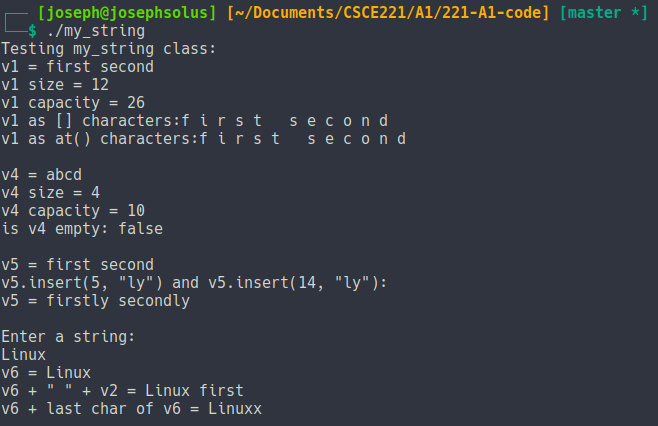
\includegraphics[scale=.7]{A1img01.png}
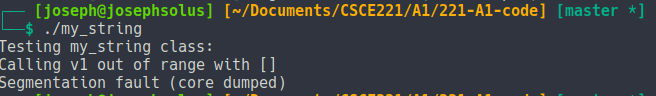
\includegraphics[scale=.7]{mystring02.png}
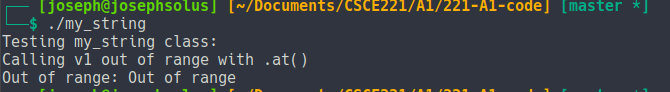
\includegraphics[scale=.7]{outofrange.png}
\end{enumerate}

\end{document}
